\section{Experiments}
\label{experiments}
\subsection{Experiments Settings}
We evaluate the system on mobile GUI tasks with screenshot-only perception. Experiments report task success rate, average steps to success, and failure breakdown by error type (grounding error, parser miss, reflection false negative, or timing-induced failure). \textcolor{red}{TODO: list the benchmarks/datasets used (e.g., GUIOdyssey if applicable), task categories, and train/val/test splits if any.}

\paragraph{Models and parsers}
Planning, action selection, and verification are performed with MLLMs, while GUI parsing produces element-level bounding boxes for grounding. \textcolor{red}{TODO: specify model names, parser version, thresholds, and any image preprocessing.}

\paragraph{Protocol}
Each task is executed with a fixed step budget and a per-step wait before capturing the next screenshot. All runs are logged with step-level traces. \textcolor{red}{TODO: define max steps, wait durations, number of trials per task, and device specs.}

\subsection{Qualitative Evaluation}
We include qualitative case studies to illustrate successful execution, recovery behavior, and failure modes. The UI screenshots you have are best placed here as a figure (or filmstrip) showing step-by-step progression. \textcolor{red}{TODO: insert figures with captions describing task goal, key actions, and where grounding or reflection succeeds/fails.}

\begin{figure}[t]
	\centering
	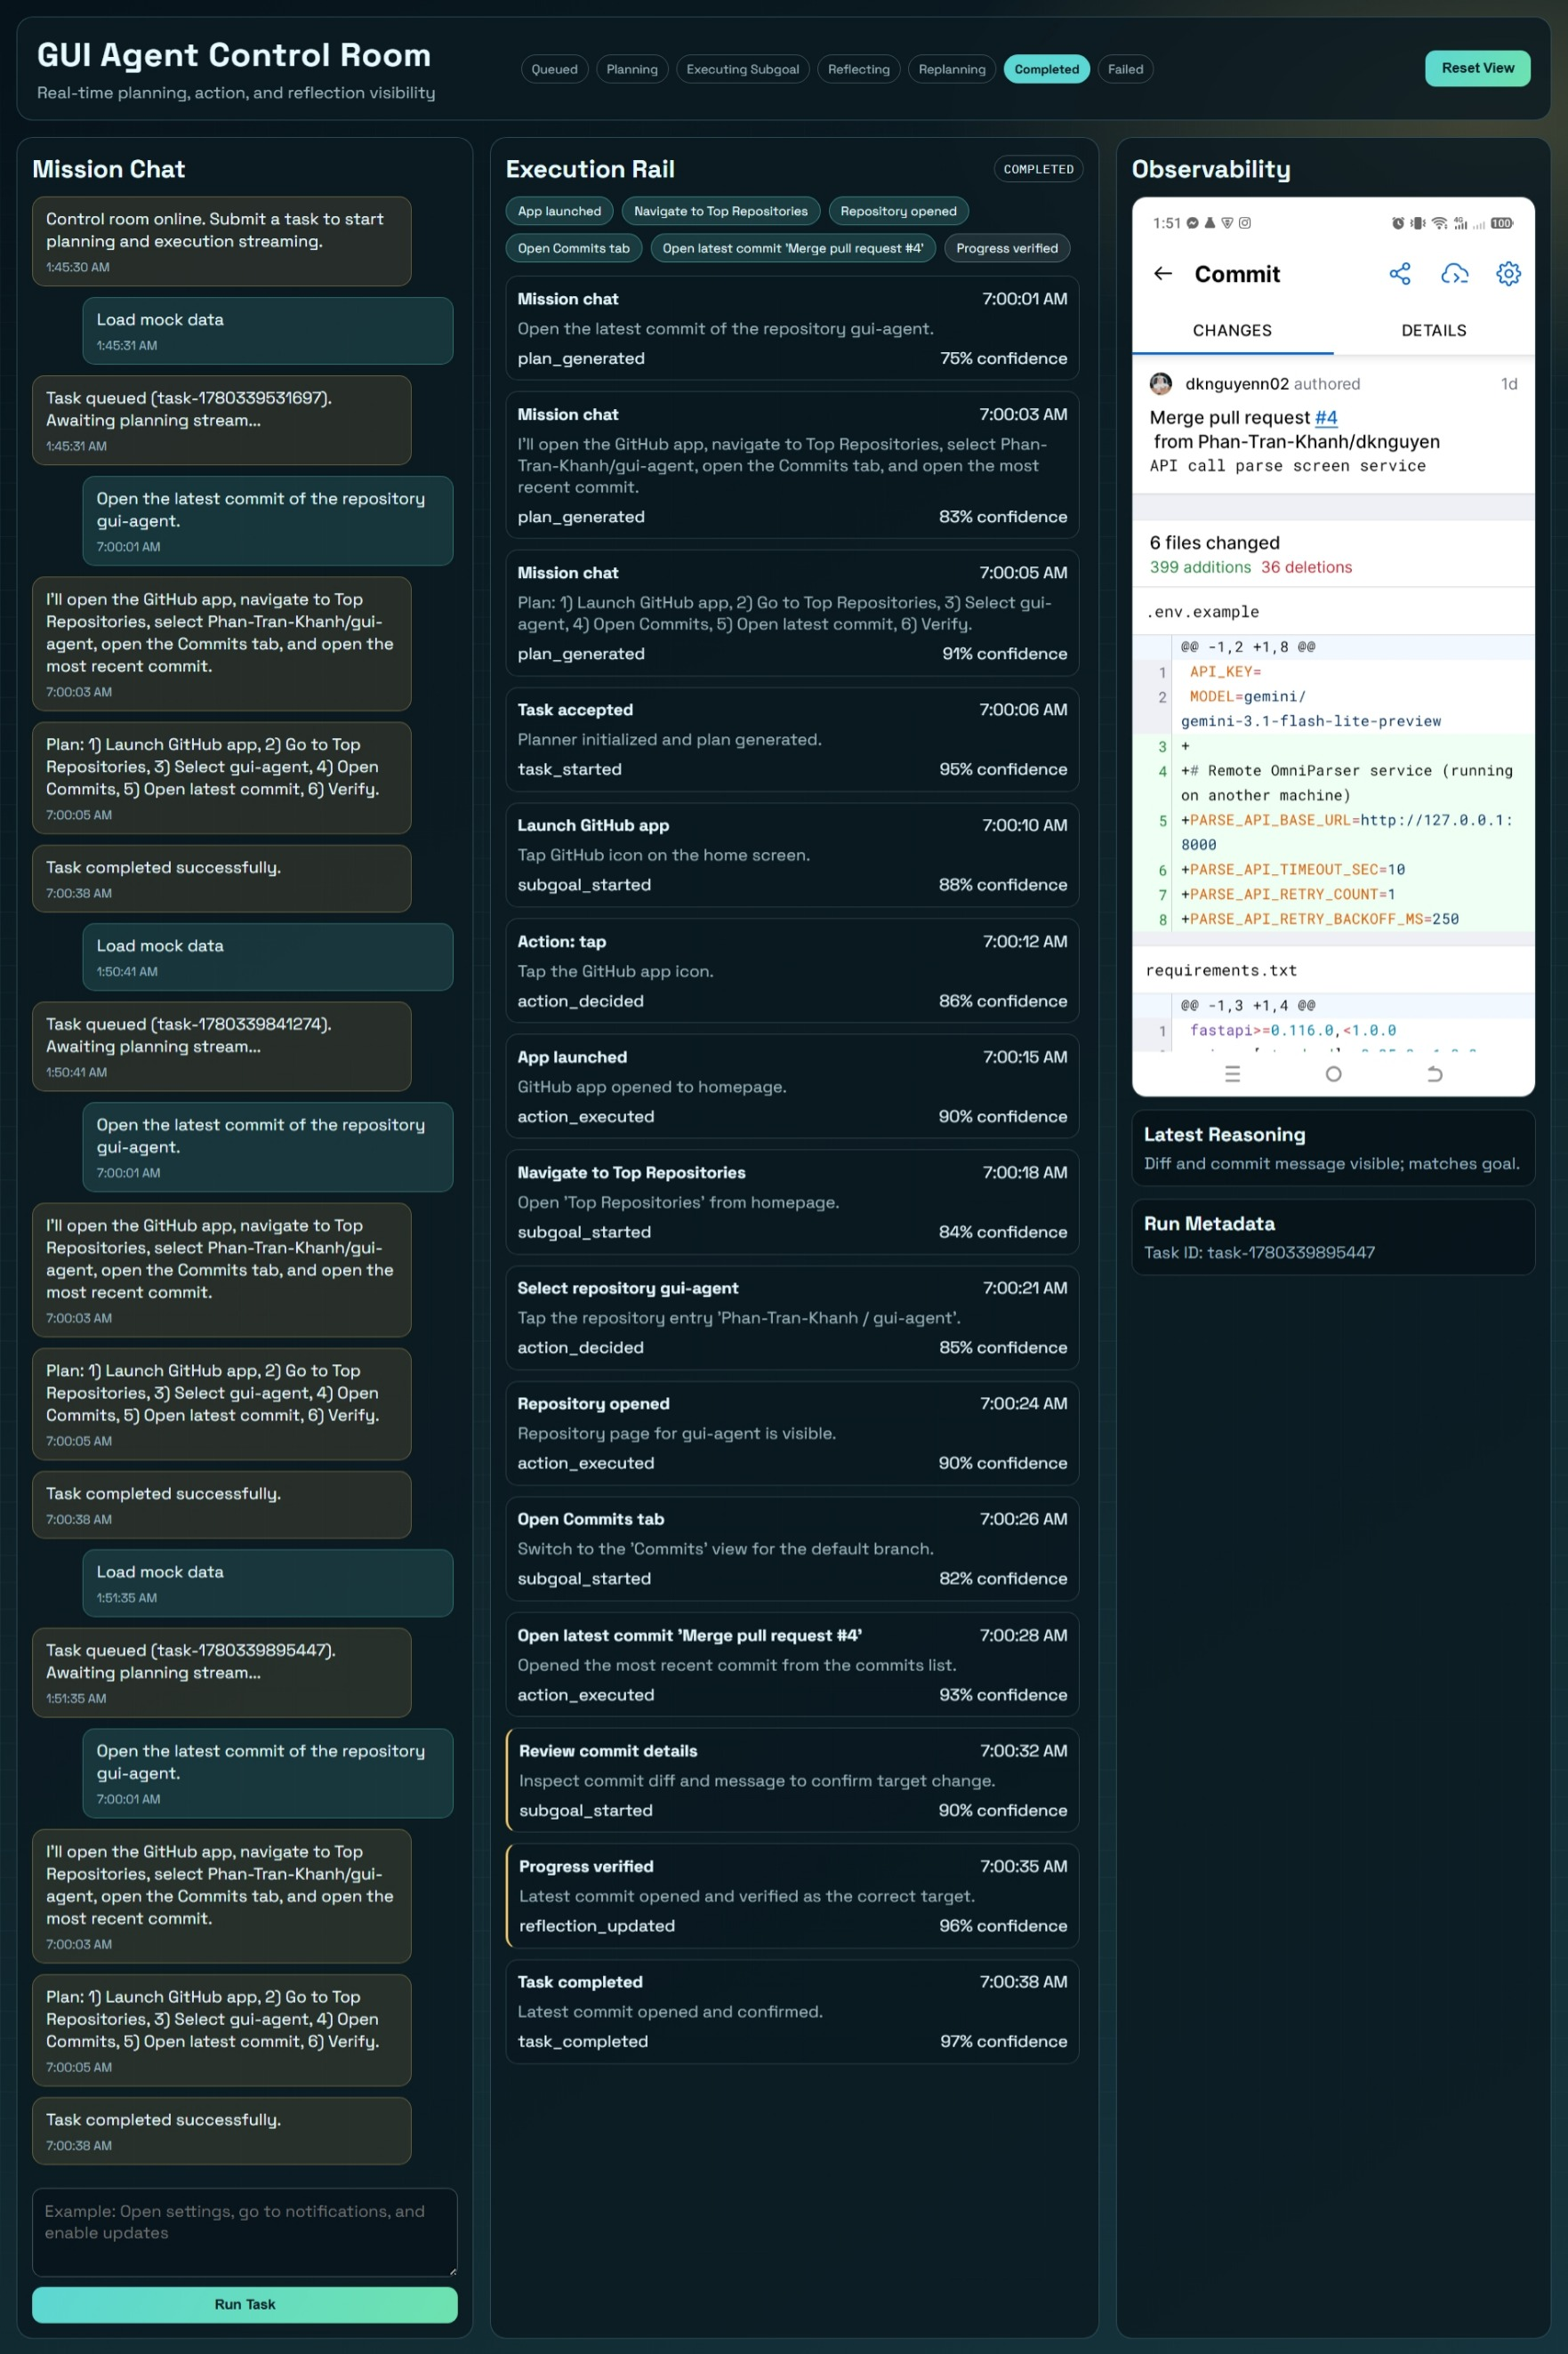
\includegraphics[width=\linewidth]{image/app-screenshot-result.jpeg}
	\caption{Example app UI screenshot from a completed run, used for qualitative inspection.}
	\label{fig:qualitative_app_ui}
\end{figure}
\subsection{Discussion}
Our experiments highlight both the practical value and the current boundaries of a grounded, screenshot-only mobile agent. When perception and grounding are reliable, the plan--act--reflect loop can complete multi-step tasks with interpretable intermediate decisions. In these cases, element-level grounding reduces obviously invalid interactions and makes failure analysis easier through step-level traces. However, several recurring failure modes suggest that robustness is still limited by reflection quality, timing assumptions, and parser coverage rather than by high-level planning alone.

\paragraph{Reflection loops on difficult screens}
A notable limitation appears on hard UI states where the agent repeatedly selects plausible but ineffective actions. The reflection stage may not recognize true sub-goal completion, while recovery proposals fail to identify a corrective target. As a result, the pipeline can remain in a local loop around the same screen region, especially when visual change is weak, transient, or visually ambiguous (e.g., subtle state toggles, loading overlays, or partially rendered widgets). In practice, execution only terminates when the per-sub-goal step budget is reached. This behavior indicates that reflection currently acts as a weak progress gate: it can detect \emph{non-progress}, but it does not always guide the agent toward the \emph{correct} progress path.

\paragraph{Timing and environment-induced failures}
Another class of failures is caused by delayed UI transitions rather than incorrect reasoning. Mobile tasks often depend on network latency, backend response time, or device performance. If a screenshot is captured before the interface stabilizes, the grounder may return incomplete or empty element sets. The planner may then infer that no valid action exists and terminate the flow early, even though the task could succeed with additional waiting. This exposes a mismatch between fixed-step control and real-world asynchrony: the current pipeline assumes near-instant UI updates, while many apps require longer transition windows.

\paragraph{Implications for system design}
These observations suggest three design priorities for future work. First, reflection should move beyond binary visual-change checks toward stronger sub-goal verification (e.g., screen-question answering or goal-conditioned state tests). Second, the controller should incorporate adaptive waiting and re-capture policies before declaring failure on sparse detections. Third, recovery should include escalation strategies when repeated attempts fail (e.g., sub-goal expansion, full replanning, or explicit user intervention), rather than relying solely on local retries within the same visual context.

Overall, the results support our central claim that explicit grounding improves controllability, but they also show that reliable mobile automation requires tighter coupling between timing, verification, and recovery. The current system provides a useful baseline for studying these trade-offs; improving long-horizon stability under delayed and ambiguous UI conditions remains an open challenge.
